%!TEX program = pdflatex
\documentclass{elegantpaper}

\title{LiteMVSNet: A Lightweight Multi-View Stereo Network with Cascade Depth Searching Scope and Recurrent Pseudo-3D CNNs}
\author{Li Yan, \href{https://fishhe.github.io/}{ Dengsu Zhang}, Hong Xie, Jin Shan \\
		SGG4DRecon Group}
\date{\small\itshape Version: 0.01 \\ Last update: \today}

\begin{document}

\maketitle

\begin{abstract}
	Various neural networks have shown that depth estimation using multi-view stereopsis can be well simulated by deep learning. The competition between running time and memory cost steps on stage. R-MVSNet, one of the state-of-the-art project, provides a gated recurrent unit (GRU) architecture to decompose 3D CNNs to 2D RNN for cost regularization, at the expense of inherent parallelism. The conflict between space and time for matching cost regularization is alliviated by our method: (1)We present an alternative network named LiteMVSNet that ourperforms R-MVSNet on the ETH3D benchmark, and requires less memory space. (2)We present a more effective depth regularization architecture with cascade depth searching scope. (3)Our networks own an efficient structure for feature extraction and cost regularization with pseudo-2D/3D CNNs. The proposed approach is compared with classic and learning-based algorithms.
\end{abstract}

\section{Introduction}
  Multi-view Stereo (MVS) methods estimates a 3D model from a collection of overlapping 2D images with known camera intrinsic and extrinsic parameters, which can be estimated by structure from motion (SFM) pipline. Stereo matching algorithms universally takes four steps: cost computation, cost regularization, depth computation and depth refinement \cite{Scharstein2001}. The matching cost can be calculated by different similarity measures\cite{Chambon2011}\cite{Chang2008}, witch are always called features in machine learning. Traditional ways have tried every effort to illustrate implicit features in MVS pipline, such as texture\cite{leibe_shading-aware_2016}\cite{7350114}, geometric structures\cite{Romanoni2019TAPAMVSTP}\cite{ShujiSAKAI}\cite{Rhemann:2011:FCF:2191740.2191908}, imaging characteristics\cite{Srinivasan2018}\cite{Zhuo:2011:DME:1994015.1994271}, and sematic cues\cite{Xu2015}. However, it seams inexhaustible to make explicit functional expressions of all these cues.

  Fortunately, the CNN structure provides an elegant way to utilize these featues which are significant for 3D reconstruction. Learning-based MVS methods recently achieve state-of-the-art performance on 3D reconstruction benchmarks\cite{jensen2014large}\cite{Knapitsch2017}\cite{schoeps2017cvpr}.

  Nevertheless, many existing learning-based MVS\cite{DBLP:journals/corr/abs-1804-00650}\cite{DBLP:journals/corr/abs-1804-02505}\cite{DBLP:journals/corr/abs-1901-01535} requires a large memory space for feature extraction and cost regularization. All of these projects use space-sweeping method\cite{517097}. The problem space grows cubically with the model resolution. Some methods are proposed for this defect: OctNet\cite{DBLP:journals/corr/RieglerUG16} and AO-CNN\cite{Wang-2018-AOCNN} apply the octree structure on 3D CNNs, as 3D data is usually sparse. R-MVSNet\cite{DBLP:journals/corr/abs-1902-10556} introduces GRU to decompose 3D CNNs into recurrent 2D CNNs, so that R-MVSNet is capable for high resolution 3D reconstruction with unlimited depth-wise resolution. At the cost of the serial structure, R-MVSNet's running time grows linearly with the size of depth dimension. It is the trade-off between space and time that this paper concerns.

  In this paper, we presents a lightweight multi-view stereo framework, named as LiteMVSNet. The framework is built upon MVSNet \cite{DBLP:journals/corr/abs-1804-02505} and DeMoN\cite{DBLP:journals/corr/UmmenhoferZUMID16} architectures, and introduces the cascade depth searching scope (CDSS) and recurrent pseudo-2D/3D CNNs (RP-CNNs) for depth inference. The depth searching scope is gradually shrinked to the truth, which helps to avoid unnecessary time cost and improves the efficiency of execution. The RP-CNNs are helpful for both decreasing the width of the model and increasing it's depth.

	DTU\cite{jensen2014large}, Tanks and Temples\cite{Knapitsch2017} and ETH3D datasets\cite{schoeps2017cvpr} are used for evaluation. We compare our method with the state-of-the-art projects: (COLMAP, DeepMVS, MVSNet, R-MVSNet, and DeepTAM). Our method has the ability for high resolution reconstruction, and is time saving for higher depth-wise resolution.


\section{Related Work}

 FlowNet\cite{7410673} and MatchNet\cite{7298948}, the pioneers to learn pair-wise matching, expand a brand new area in deep learning. Before long, FlowNet2\cite{DBLP:journals/corr/IlgMSKDB16}, DispNet\cite{MIFDB16}, and SGMNet\cite{MIFDB16} achieve to exceed non-learning method in early vision tasks (such as flow estimation, disparity computation and patch matching). DeMoN\cite{DBLP:journals/corr/UmmenhoferZUMID16}, mainly based on the idea of FlowNet2, clearly demonstats how to establish the correspondence for two-view geometry. However, expanding two-view to multi-view for learning-based method is a demanding work. It is not only a challenge in function modeling but also a dramatical increase in computing requirements.

 Space-sweeping\cite{517097} (or plane-sweeping\cite{4270270}) is the mainly technique employed in current MVS networks. There're three steps in space-sweeping: cost volume computation, cost regularization, and depth inference.

 The mathing cost is defined by the similarity metrics. Almost all the learning-based architectures use 2D CNNs to extract features for similarity computation, but some, like DeepTAM\cite{ZUB18}, use traditional metrics for efficiency and astringency. SurfaceNet\cite{DBLP:journals/corr/abs-1708-01749} introduces colored voxel cube (CVC) for cost computation with multi view stereopsis. However, it accumulates the cost in object space, which makes the method incapable for large scale scenes. MVSNet introduces a differentiable homography warping, so that cost volume can be computed in image space. In this way, the space can be only sweeped with planes. A more generalized nonlinear warping using flow can be found in the series of LMB's works\cite{ISKB18}\cite{ZUB18}. Flow-warping is the key to our CDSS, which makes it possible to arbitrarily sweep the space.

 There are mainly two ways to regularize the cost volume and infere the depth map: 2D CNNs and 3D CNNs. Matching costs, which are calculated at different depth of a same pixel, can be feed into 2D CNNs' feature channle. This trick is used by DeMoN, DeepMVS and DeepTAM. In addition, some projects, like MVSNet and R-MVSNet, use 3D CNNs, which give the cost volume a more distinct geometry interpretation. The method with 2D CNNs discards the inherent 3D data structure, and forces the model to learn it. Despite the model's ability to express the geometry, additional memory costs are caused. Unlike 2D CNNs, 3D CNNs only make local links in depth dimension,

 The skeleton structure of learned MVS has been developed by previous works. However, most of them ask for a large quantity of GPU memory. DeepMVS, which uses extremely high-dimensional features (VGGNet19\cite{Simonyan14c}), can only handle 128px $\times$ 128px patches (the center of 64px $\times$ 64px used for tiling) with 4GB memory at once. The whole input image is splitted into patches, and then outputs are tiled to achieve full-resolution result. It takes around 4s for a patch on 1080Ti, and 4min for the whole image of 512px $\times$ 512px, which is unacceptable for practical application. Same shortcomings exist in other 2D-CNNs-based structures. 3D CNNs are much more time-saving but also memory-expensive. R-MVSNet introduces the GRU structure to sequentially regularizes the 2D cost maps along the depth direction. By this way, R-MVSNet reduces the memory consumption at the expense of running time. However, the GRU doesn't break the local link structure in depth dimension, so it is still more efficient both in space and time than 2D CNNs. 


\section{LiteMVSNet}

In this section, we will describe the

\subsection{Network Outline}

\subsection{Features}

\subsection{Cost Volume}

\subsection{Depth Map}

\subsection{Loss}


\section{Experiment}




\section{Related Work}



\subsection{Font Settings}
I change the default article font computer modern to \verb|newtx| series, and the default font size is set to \verb|11pt|.

\begin{itemize}[noitemsep]
	\item \verb|newtxtext| package for text font, similar to times new roman font.
	\item \verb|newtxmath| package for math font, close to \verb|times| and \verb|mtpro2| packages.
	\item \verb|newtxtt| package for typewriter font, with option \verb|scale = 0.8|.
\end{itemize}

These packages operate perfectly but are inappropriate for big operators, for example \verb|\sum| and \verb|\prod|, thus, I change these operators back to computer modern font. Equation~\eqref{eq:binom} shows the effects of these fonts:
\begin{equation}
(a+b)^{n} = \sum_{k=0}^{n} C_{n}^{k} a^{n-k} b^k \label{eq:binom}
\end{equation}



The \verb|\linespread| (controls line spacing) is set to 1.3, and I use \verb|microtype| to improve the font justification. \verb|type1cm| package is used to remove the font shape and font size warning messages.

\subsection{Custom Commands}

I don't change any default command or environment, which means you can use all the basic \LaTeX{} commands and environments as before.  Besides, I define 3 commands
\begin{enumerate}[noitemsep]
	\item \verb|\email{#1}|: create the hyperlink to email address.
	\item \verb|\figref{#1}|: same usage as \verb|\ref{#1}|, but start with label text <\textbf{Figure n}>.
	\item \verb|\tabref{#1}|: same usage as \verb|\ref{#1}|, but start with label text <\textbf{Table n}>.
\end{enumerate}{}

\subsection{List Environments}
When you are using \verb|itemize|, \verb|enumerate|, or \verb|description| environment, please add the \verb|noitemsep| option to these environments. For example, \\

\begin{minipage}[c]{0.45\linewidth}
\begin{Verbatim}[tabsize=4,frame=single,baselinestretch=1]
\begin{itemize}[noitemsep]
	\item Routing and resource discovery;
	\item Resilient and scalable networks;
	\item Distributed storage and search.
\end{itemize}
\end{Verbatim}
\end{minipage}
\begin{minipage}[c]{0.45\linewidth}
\begin{itemize}[noitemsep]
	\item Routing and resource discovery;
	\item Resilient and scalable computer networks;
	\item Distributed storage and search.
\end{itemize}
\end{minipage}

\subsection{Table}
I strongly recommend you to use the \verb|booktabs| package in your paper. It adds three commands to make the table prettier, ie. \verb|\toprule|, \verb|\midrule| and \verb|\bottomrule|. Here is an example.

\begin{table}[!htbp]
  \small
  \centering
  \caption{Regression Result Example}
    \begin{tabular}{lll}
    \toprule
          & \multicolumn{1}{c}{(1)} & \multicolumn{1}{c}{(2)} \\
      & \multicolumn{1}{c}{price} & \multicolumn{1}{c}{price} \\
    \midrule
    mpg   & \multicolumn{1}{c}{-238.9***} & \multicolumn{1}{c}{-49.51} \\
          & \multicolumn{1}{c}{(53.08)} & \multicolumn{1}{c}{(86.16)} \\
    weight & \multicolumn{1}{c}{} & \multicolumn{1}{c}{1.747***} \\
          & \multicolumn{1}{c}{} & \multicolumn{1}{c}{(0.641)} \\
    constant & \multicolumn{1}{c}{11,253***} & \multicolumn{1}{c}{1,946} \\
          & \multicolumn{1}{c}{(1,171)} & \multicolumn{1}{c}{(3,597)} \\
    observations & \multicolumn{1}{c}{74} & \multicolumn{1}{c}{74} \\
    R-squared & \multicolumn{1}{c}{0.220} & \multicolumn{1}{c}{0.293} \\
    \midrule
    \multicolumn{3}{l}{\scriptsize Standard errors in parentheses} \\
    \multicolumn{3}{l}{\scriptsize *** p<0.01, ** p<0.05, * p<0.1} \\
    \end{tabular}%
  \label{tab:reg}%
\end{table}%



\subsection{Graphics}
To include a graphic, you can use figure environment as usual. \figref{fig:mpg} shows the effect. You can put all your images in the sub directories (\verb|./image/|, \verb|./img/|, \verb|./figure/|, \verb|./fig/|) of your current working directory.

\begin{Verbatim}[tabsize=4,frame=single,baselinestretch=1]
\begin{figure}[!ht]
	\centering
	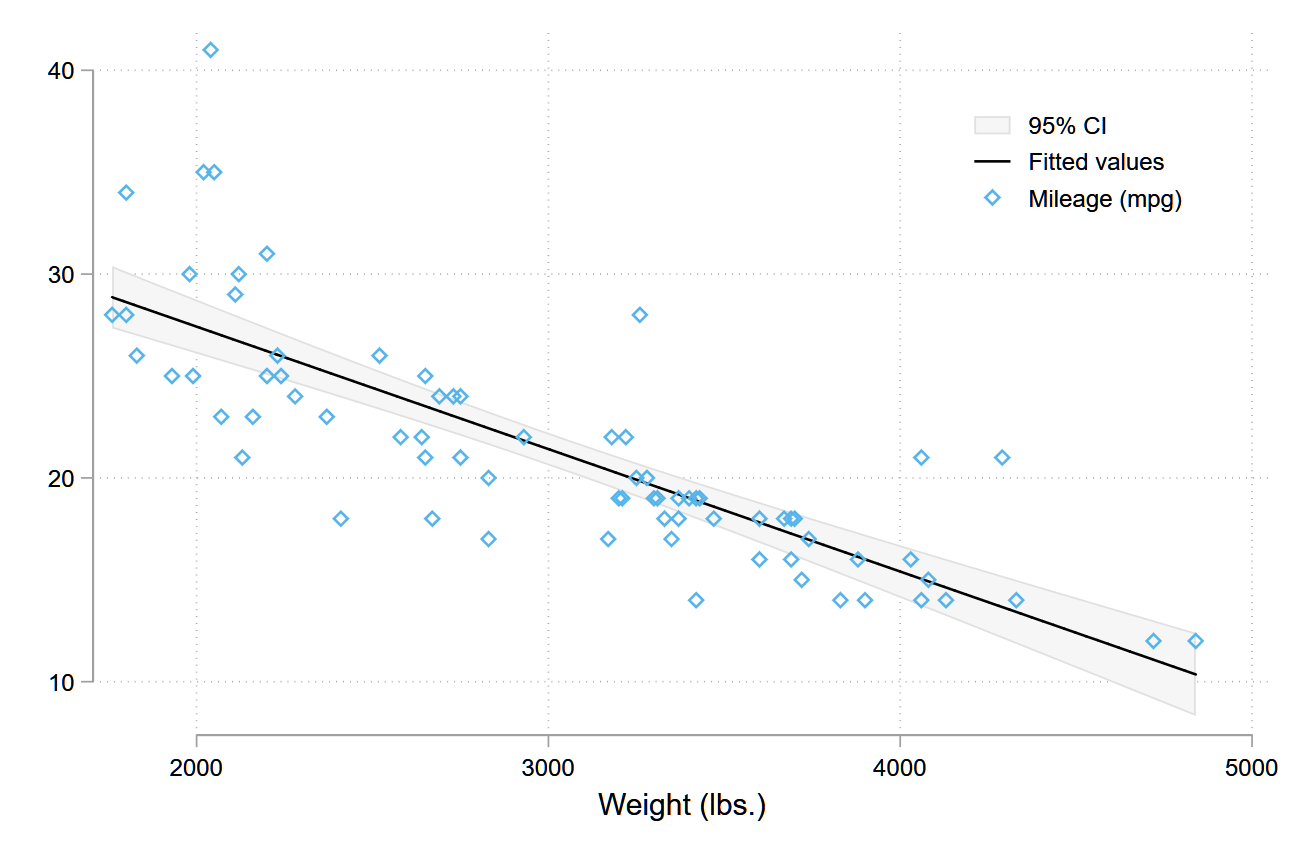
\includegraphics[width=0.6\textwidth]{mpg.png}
	\caption{The Relationship between MPG and Weight\label{fig:mpg}}
\end{figure}
\end{Verbatim}
\begin{figure}[!ht]
	\centering
	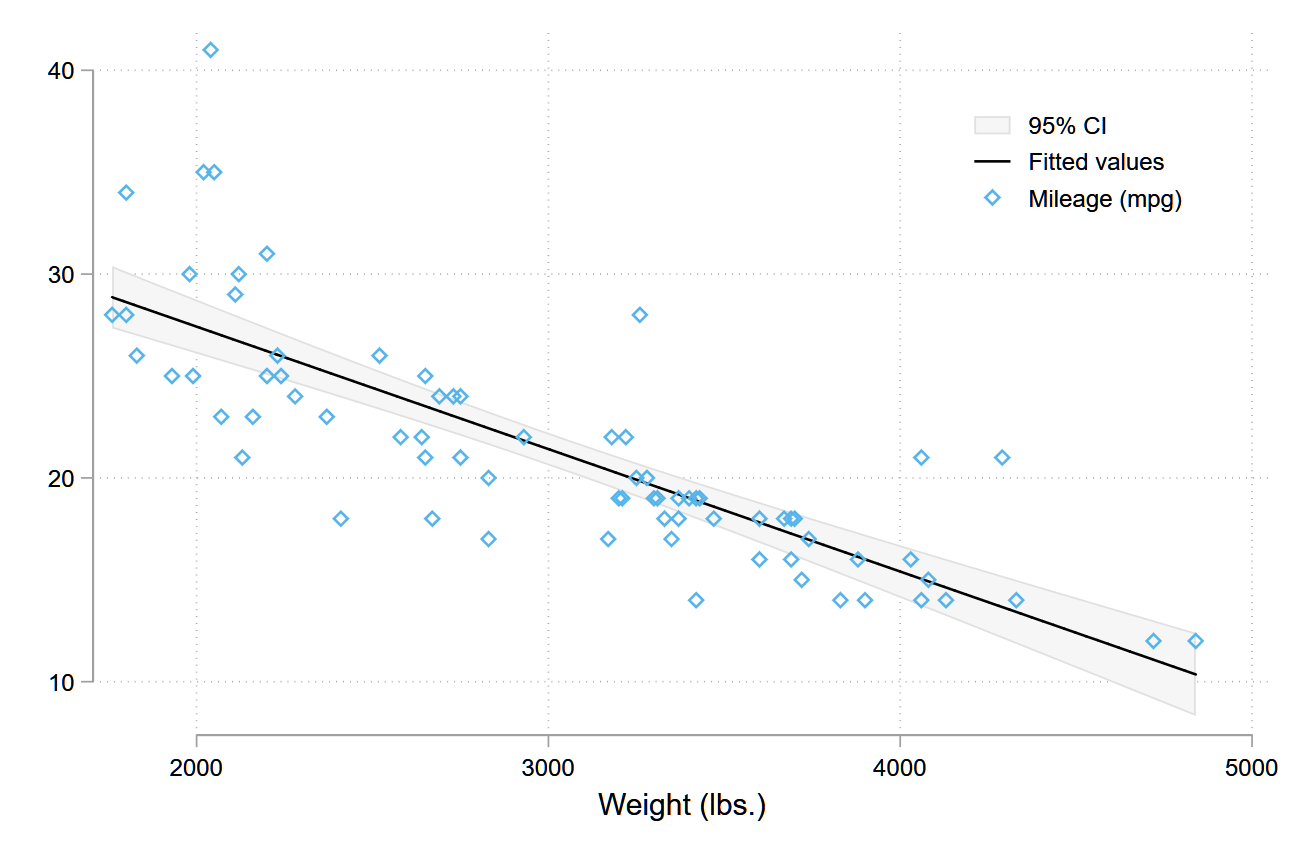
\includegraphics[width=0.6\textwidth]{mpg.png}
	\caption{The Relationship between MPG and Weight\label{fig:mpg}}
\end{figure}

\subsection{Bibliography}
This template uses Bib\TeX{} to generate the bibliography, the default bibliography style is \verb|aer|. ~\cite{Chen2018} use data from a major peer-to-peer lending marketplace in China to study whether female and male investors evaluate loan performance differently. You can add bib items (from Google Scholar, Mendeley, EndNote, and etc.) to \verb|wp_ref.bib| file, and cite the bibkey in the \verb|tex| file.


\nocite{EINAV2010,Havrylchyk2018}

\bibliographystyle{plain}
\bibliography{wp_ref}
\end{document}
